\documentclass[journal]{IEEEtran}
\IEEEoverridecommandlockouts
% The preceding line is only needed to identify funding in the first footnote. If that is unneeded, please comment it out.
\usepackage{cite}
\usepackage{amsmath,amssymb,amsfonts}
\usepackage{algorithmic}
\usepackage{graphicx}
\usepackage{textcomp}
\usepackage{xcolor}
\usepackage{subfig}
\usepackage[export]{adjustbox}
\def\BibTeX{{\rm B\kern-.05em{\sc i\kern-.025em b}\kern-.08em
    T\kern-.1667em\lower.7ex\hbox{E}\kern-.125emX}}
\begin{document}

\title{Explore and Protect a location\\
{\footnotesize Final Project - ECE6563 Networked Control Systems - Fall 2018}
}

\author{\IEEEauthorblockN{Vincent \textsc{Maffet}}
\IEEEauthorblockA{\textit{Electrical and Computer Engineering} \\
\textit{Georgia Institute of Technology}\\
Metz, France \\
vincent.maffet@gatech.edu}
}

\markboth{Explore and Protect a location, November 2018}{Explore and Protect a location, November 2018}

\maketitle
\thispagestyle{empty}

\begin{abstract}
This documents explains how to protect a flag/location with multiple agents. This is achieved through Gabriel triangulation and Voronoi partitions. The agents are controlled in a local, scalable, safe/reactive and emergent way, answering the key issues of networked control systems.
\end{abstract}

\begin{IEEEkeywords}
CTF, Voronoi, Gabriel
\end{IEEEkeywords}

\section{Introduction}

The setting of the experiment is a game called Capture the Flag.\\

This is a very popular game. It is played in multiple environments, from playgrounds to video games, not to mention hacking competitions.\\
We will now make robots play this game.\\

As a reminder, the rules are the following:
\begin{itemize}
    \item 2 teams confronting
    \item Each team has one flag
    \item Each team must find, steal and retrieve the opponent's flag, while protecting its own flag
\end{itemize}
\ \\
In this document we will focus on the task of protecting the flag.
To achieve this we will secure the area around it.
Each agent will secure and monitor a piece of land by standing in the middle of it.\\

In the following sections we will detail the control protocols and how we ensure the security of our flag. 

\section{Global behavior}

In order to secure our flag from attackers, we will station multiple agents surrounding it.\\
With a formation like that, opponents will be identified and stopped before they could do anything.\\

Our strategy has multiple states and will switch between them at the right time.\\

First the security agents are looking to get together near the flag.
Then we have two behaviors.\\
Our agents can either execute a close protection around the flag or cover the whole space around it to look for potential threats in a patrolling way.\\

The agents go from a close protection to a patrol protocol when they stop moving.
This way the agents are always on the move, making it harder for the attackers to find a breach and sneak in-between guards.\\
Also by expanding and grouping, the agents are doing a breathing movement, thanks to this we are more confident in reaching a 'stable' optimal state. 

\section{Close protection}

Ensuring a close protection of the flag is essential. We have plenty of reasons to do it. For instance in case of an incoming attack you would want your guards to gather around and closely protect the flag.\\
It is a very secure way of protecting an asset. You have to defeat plenty of agents before accessing the flag, with no other way around.

\subsection{Assumptions}

For our protocol to work, we need to lay some assumptions about the robots.\\

We will need to have a way of detecting other robots and the flag.
This could be achieved with some basic sensors like infrared or ultrasound range sensors.\\

One important point is that the robots need to identify their allies securely and reliably. For this we need some communication. We can use some short range standard like Bluetooth depending on the distances scale of the environment. The communications are then secured with cryptography protocols like zero-knowledge proofs to ensure that you are talking to allies.\\

To recap we have some range sensors to detect entities and a communication device to identify them.

\subsection{Implementation}

The close protection of the flag is done by doing a near-coverage through Gabriel Graphs.\\

Gabriel Graphs are an efficient way to find the nearest neighbors interaction graph. When knowing the according connections between agents, we are able to compute a triangulation.\\
The generated triangulation is not perfect but it is quick and light to compute and can be done in a local, scalable and reactive way.
Those are important properties when in a danger situation. You do not want to rely on a central unit which could be compromised. You also want to converge fast and be resilient to the loss of some agents on the battlefield.\\

To compute the graph (hence the edges), we take two agents $a_i,a_j$ and check if the circle of diameter $||a_i-a_j||$, passing through $a_i$ and $a_j$ contains any other agent. If there is no agents inside the circle, then there is an edge between $a_i$ and $a_j$ in the Gabriel Graph.
The figure \ref{gab_edge} illustrates the test.\\
\begin{figure}
	\centering
	\subfloat[Valid Edge]{{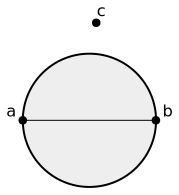
\includegraphics[width=3cm]{../images/paper/Gabriel_Pairs.png} }}
	\qquad
	\subfloat[Invalid Edge]{{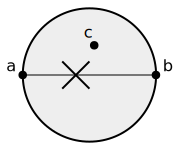
\includegraphics[width=3cm]{../images/paper/Not_Gabriel_Pairs.png} }}
	\caption{Computing Gabriel Graph edges}
	\label{gab_edge}
\end{figure}

Once we know the edges of the graph we apply a standard formation control law:
\begin{equation}
\dot{x_i}(t) = - \sum_{j \in {N_G}_i} \frac{||x_i(t)-x_j(t)||-\Delta}{||x_i(t)-x_j(t)||}*(x_i(t)-x_j(t)) \label{eq1}
\end{equation}

With this control law, we achieve a rigid triangulation. The agents are densely covering the area. The figure \ref{gab_sim} shows the computed edges and resulting triangulation.\\
\begin{figure}
	\centering
	\subfloat[Simulation]{{\adjincludegraphics[trim={{.13\width} {.17\height} {.09\width} {.1\height}}, clip, width=6.5cm]{../images/simulation/gabriel_sim.png}  }}
	\qquad
	\subfloat[Experimentation]{{\adjincludegraphics[trim={{.24\width} {.25\height} {.30\width} {.29\height}}, clip, width=6.5cm]{../images/experiment/gabriel_exp2.png}  }}
	\caption{Gabriel Graph Triangulation}
	\label{gab_sim}
\end{figure}

However, we are not sure that the agents are centered around the flag. Still this is not a problem. Indeed, since we periodically switch between the patrolling protocol and the close protection, the agents end up around the flag. This is due to the fact that the patrol is covering the area while being centered around the point of interest has we will see in the next section.

\subsection{Notes and References}

In this section, the necessary theoretic foundations and control laws come mainly from the recommended textbook of ECE6563 \cite{b1}.\\

Another way to gain confidence in being around the flag would be to treat it has an agent taking part in the formation.

\section{Patrol}

When no immediate threat is detected, it is a good idea to explore the area around the flag while keeping some agents near it. In a realistic scenario it makes more sense. For instance, if the flag is kept in a warehouse, on a hill or in a forest, it would be wise to send some agents explore the surroundings to make sure that the opponent isn't approaching and/or doing something.\\

This is our second way of protecting the asset. We assign areas to cover for the agents. We still want some of our agents to cover the flag closely, hence we have an importance parameter. It is critical to cover the land near the flag. Hence the further you are from the flag, the more land you can check because it is not has necessary to check the space thoroughly.

\subsection{Assumptions}

Once again we need to lay some assumptions about the robots.\\

For starters we have the ones from the previous case: our robots are equipped with range sensors and a communication device to detect and identify entities.\\

Our robots now have the much harder task of computing the area they are responsible of and its weight. This can be done partially on board with some assumptions. In our case we will use a central unit (located in the flag for instance) which knows the location of every agent and can give the right orders to the space efficiently.\\

It is not critical to rely on a central unit since this stage is more relaxed. Indeed we assumed that there is no ongoing attack and that we are sending scouts to detect enemies. Upon detecting an attack we would get back to a close protection of the flag, which is fully local.

\subsection{Implementation}

We will use a Voronoi-based coverage algorithm with a density function over the space.
The maximum of the density being at the flag location.\\

Voronoi Diagrams are a great way to assign areas to agents such that every one has the same responsibility. By weighting the areas, we make sure that each guard has the same level of danger in his zone.
\  \\\\
We considered two density functions to weight the areas: 
\begin{itemize}
	\item The inverse of the distance. This has the nice property of being infinite at the flag location. On the other hand it is not that nice since the function is quickly nil when going away from the flag.
	\begin{equation}
	\phi(x,y) = 1/\sqrt{x^2 + y^2} \label{eq2}
	\end{equation}
	\item A Gaussian distribution. This function also has the required properties. We can put the max on the flag location, then the function decreases in a nice way. We can also change $\sigma$ to set the importance range.
	\begin{equation}
	\phi(x,y) = \exp(-\sqrt{x^2 + y^2}^2/\sigma^2) \label{eq3}
	\end{equation}
\end{itemize} 

Figures \ref{weight_inv} and \ref{weight_gauss} are a representation of the weights and the according simulation results.

\begin{figure}
	\centering
	\subfloat[Density mapping]{{\includegraphics[width=5cm]{../images/paper/inv_density.png}  }}
	\quad
	\subfloat[Voronoi diagram]{{\adjincludegraphics[trim={{.13\width} {.17\height} {.09\width} {.1\height}}, clip, width=5cm]{../images/simulation/voronoi_sim_inv.png}  }}
	\caption{Inverse density}
	\label{weight_inv}
\end{figure}

\begin{figure}
	\centering
	\subfloat[Density mapping]{{\includegraphics[width=5cm]{../images/paper/gauss_density.png}  }}
	\quad
	\subfloat[Voronoi diagram]{{\adjincludegraphics[trim={{.13\width} {.17\height} {.09\width} {.1\height}}, clip, width=5cm]{../images/simulation/voronoi_sim_gauss.png}  }}
	\caption{Gaussian density}
	\label{weight_gauss}
\end{figure}

From the simulations, and because of the flexibility of the $\sigma$ parameter, I think that the Gaussian function yields better results for our problem. We will discuss this again in the next section.\\

About the implementation of the algorithm. We apply a control law which we got from doing a gradient decent on the locational cost with the density function. Hence we implemented this law:
\begin{equation}
\dot{x_i}(t) = - \int_{\nu_i} \phi(q)*(x_i(t) - q) dq \label{eq4}
\end{equation}

To compute the integral we used numerical integration, specifically the middle Riemann sum. It allows us to easily compute the integral while having a relatively small error.

\subsection{Notes and References}

In this section we mainly discussed Voronoi partitions. In order to understand the theoretic foundation and how the control law arises from it we mainly based ourselves on the recommended textbook of ECE6563 \cite{b2}.\\

In our implementation we computed the neighbors thanks to a delta-disk for the initial consensus and the Gabriel triangulation. We could have pushed the analogy further and used r-limited Voronoi cells \cite{b3} to have a less centralized system.\\  

The numerical integration can be understood in depth thanks to this calculus book \cite{b4}.

\section{Results}

We now have all the details of our protocol to protect the flag.\\

It starts with a rendez-vous at the flag location (Blue dot in simulations). Then it does a Gabriel triangulation. After achieving it, when the danger is away, the agents start to do a weighted Voronoi coverage. When a stable formation is found, we switch back to a Gabriel triangulation has if we were getting attacked and so on.\\

The Gabriel triangulation works perfectly, the required distances are correctly set between agents and we can see edges updating thanks to the circle rule.\\

The Voronoi partition is trickier. We tested two density functions. The Gaussian one seems to be the best. With nine agents we keep two around the flag while the others are going to check the surroundings. In the inverse function we don't see much of a difference. There is notably one agent which goes on top of the flag, but the rest of the agents split the remaining space evenly. This is not what we want. The aim is not to give the same amount of space but the same amount of dangerousness. And being close to the flag should give you higher responsibility hence less space to look out for.\\

One of the biggest discrepancy between the simulations and the experiments is the Voronoi coverage. The primitive space element used to do the numerical integral needs to be smaller in the experiments. In reality, the robots are controlled less precisely and not in a discrete way. Hence they tend to oscillate because of space elements switching between agents. To avoid the oscillations we just need to set a smaller integration step. However we can see this as an unexpected feature, it makes each agents do small loops, making it easier for them to spot everything in their area. Figure \ref{vrn_exp} shows an experimental coverage.\\
\begin{figure}
	\centering
	\adjincludegraphics[trim={{.07\width} {.05\height} {.165\width} {.11\height}}, clip, width=5.52cm]{../images/experiment/voronoi_exp.png}
	\caption{Experimental Voronoi coverage}
	\label{vrn_exp}
\end{figure}


One nice result about our protocol is that it does not care about the number of robots. We can change it easily and get the best coverage possible. It is still a good idea to get a good number of robots to have a nice coverage of the zone has we can see in figure \ref{vrn_nba}. I would not put less than seven robots since this is when we start having agents staying near the flag while others go further.
\begin{figure}
	\centering
	\subfloat[2 agents]{{\adjincludegraphics[trim={{.13\width} {.17\height} {.09\width} {.1\height}}, clip, width=4cm]{../images/simulation/voronoi_2.png}  }}
	\quad
	\subfloat[5 agents]{{\adjincludegraphics[trim={{.13\width} {.17\height} {.09\width} {.1\height}}, clip, width=4cm]{../images/simulation/voronoi_5.png}  }}
	\quad
	\subfloat[7 agents]{{\adjincludegraphics[trim={{.13\width} {.17\height} {.09\width} {.1\height}}, clip, width=4cm]{../images/simulation/voronoi_7.png}  }}
	\quad
	\subfloat[13 agents]{{\adjincludegraphics[trim={{.13\width} {.17\height} {.09\width} {.1\height}}, clip, width=4cm]{../images/simulation/voronoi_13.png}  }}
	\quad
	\subfloat[25 agents]{{\adjincludegraphics[trim={{.13\width} {.17\height} {.09\width} {.1\height}}, clip, width=5.1cm]{../images/simulation/voronoi_25.png}  }}
	\caption{Coverage with different number of agents}
	\label{vrn_nba}
\end{figure}

Another perk of our protocol is that we never had to do any assumptions about the environment, once the agents have found the flag they protect it effectively.\\

Also it would integrate well with the other parts of the game. Lets say that we have another protocol which goes and retrieves the enemy flag. Upon their return, they will be autonomously considered part of the formation by the protecting agents.

\section{Conclusion}

Our control protocol answers the issues of the protection stage in a Capture the Flag game played by robots.\\

We came up with an elegant solution, making use of the numerous robots and relying on their cooperation. In critical moments we satisfy all the conditions of a good networked system, being local, scalable, safe/reactive and emergent.\\

Thanks to a rendez-vous with every agent and the flag all the agents are meeting around the place to defend.\\
Then we have two alternating behaviors. A very defensive one with the Gabriel triangulation, giving us a near-coverage of the flag, making it impossible for the opponent to breach the protection. And a scouting one, which assigns the dangerous areas in a smarter way to explore the direct surrounding while still protecting the flag.\\

By switching between the two states we increase our security, making our behavior less predictable to the enemy.\\

Now that we built the framework, we can imagine more sophisticated formations thanks to the density function of the Voronoi coverage.


\begin{thebibliography}{00}
\bibitem{b1} M. Mesbahi and M. Egerstedt, ``Graph Theoretic Methods in Multiagent Networks'', Princeton University Press, 2010, pages: 180--183.
\bibitem{b2} M. Mesbahi and M. Egerstedt, ``Graph Theoretic Methods in Multiagent Networks'', Princeton University Press, 2010, pages 184--188.
\bibitem{b3} S. Martinez, J. Cortés, and F. Bullo, ``Motion coordination with distributed information'', IEEE Control Systems Magazine, 2007, pages: 75--88.
\bibitem{b4} A. Ostebee and P. Zorn, ``Calculus from Graphical, Numerical, and Symbolic Points of View'', W.H. Freeman, Second Edition, 2002, pages: M 33--34.
\end{thebibliography}

\end{document}
